\section{Virtual Detector Architecture}

\subsection{The Nature of Virtual Detectors}

\begin{definition}[Virtual Detector]
\label{def:virtual_detector}
A virtual detector $\mathcal{D}_{\text{virtual}}$ is a measurement device that exists as a categorical construct only during the act of measurement. It is \textbf{not} persistent hardware but a transient information processing structure materialized from the underlying MMD categorical state at a convergence node.

Formally:
\begin{equation}
\mathcal{D}_{\text{virtual}} = \begin{cases}
\text{MMD}(\mathbf{S}_{\text{cat}}, \mathcal{C}_{\text{node}}, \mathcal{P}_{\text{instrument}}) & \text{during measurement} \\
\emptyset & \text{otherwise (non-existent)}
\end{cases}
\label{eq:virtual_detector_existence}
\end{equation}

where:
\begin{itemize}
    \item $\mathbf{S}_{\text{cat}}$ is the categorical state captured at convergence node
    \item $\mathcal{C}_{\text{node}}$ is the convergence node location (scale, frequency, phase)
    \item $\mathcal{P}_{\text{instrument}}$ is the instrument projection operator (TOF, Orbitrap, FT-ICR, etc.)
\end{itemize}
\end{definition}

\begin{axiom}[Transient Existence Principle]
\label{axiom:transient_existence}
Virtual detectors have no persistent physical embodiment. They exist only as information processing operations applied to categorical states during measurement events. Between measurements, no detector structure exists—neither physically nor informationally.

This is fundamentally different from:
\begin{itemize}
    \item \textbf{Physical detectors}: Persistent hardware (photomultiplier tubes, MCPs, Faraday cups) that exist continuously
    \item \textbf{Simulated detectors}: Software models that persist as code/data structures
    \item \textbf{Virtual detectors}: Emerge only when needed, dissolve immediately after
\end{itemize}
\end{axiom}

\begin{remark}[Why Virtual Detectors Work]
Three principles justify virtual detector operation \citep{ultra_high_resolution_interferometry}:

\textbf{(1) Screen Principle}: In quantum mechanics, measurement is fundamentally about correlations between system and apparatus states, not physical interaction. The "screen" (detector) can be any system capable of registering correlations.

\textbf{(2) Categorical State Completeness}: The categorical state $\mathbf{S}_{\text{cat}}$ at a convergence node contains complete information about molecular observables—not trajectories, not intermediate states, but \textit{measurement outcomes}.

\textbf{(3) Zero Backaction}: Reading categorical states has zero quantum backaction because categorical positions are already occupied (Axiom \ref{axiom:categorical_irreversibility}). We're not forcing a quantum collapse—we're reading a completed categorical transition.

Together: Virtual detectors "read" pre-existing categorical information without physical interaction, hence require no persistent hardware.
\end{remark}

\subsection{Virtual Detector Architecture Components}

\begin{definition}[Virtual Detector Architecture]
\label{def:virtual_detector_architecture}
A virtual detector consists of four logical components:

\begin{equation}
\mathcal{D}_{\text{virtual}} = \{\mathcal{M}_{\text{core}}, \mathcal{R}_{\text{cat}}, \mathcal{P}_{\text{inst}}, \mathcal{V}_{\text{output}}\}
\label{eq:detector_components}
\end{equation}

where:

\textbf{(1) MMD Core} ($\mathcal{M}_{\text{core}}$): Dual filtering operator implementing:
\begin{align}
\Im_{\text{input}}: &\quad \Omega^{\text{POT}}_{\text{cat}} \to \Omega^{\text{ACT}}_{\text{selected}} \\
\Im_{\text{output}}: &\quad \Omega^{\text{ACT}}_{\text{selected}} \to \Omega^{\text{VALID}}_{\text{hardware}}
\end{align}

\textbf{(2) Categorical State Reader} ($\mathcal{R}_{\text{cat}}$): Reads S-entropy coordinates and categorical position at convergence node:
\begin{equation}
\mathcal{R}_{\text{cat}}: \mathcal{C}_{\text{node}} \to \mathbf{S}_{\text{cat}} \in \mathbb{R}^{14}
\end{equation}

\textbf{(3) Instrument Projection} ($\mathcal{P}_{\text{inst}}$): Maps categorical state to instrument-specific observables:
\begin{equation}
\mathcal{P}_{\text{inst}}: \mathbf{S}_{\text{cat}} \to \mathbf{X}_{\text{instrument}}
\end{equation}
Examples: $\mathcal{P}_{\text{TOF}}$, $\mathcal{P}_{\text{Orbitrap}}$, $\mathcal{P}_{\text{FT-ICR}}$, $\mathcal{P}_{\text{IMS}}$

\textbf{(4) Validation & Output} ($\mathcal{V}_{\text{output}}$): Enforces hardware coherence constraints and formats output:
\begin{equation}
\mathcal{V}_{\text{output}}: \mathbf{X}_{\text{instrument}} \to \text{Spectrum}_{\text{validated}}
\end{equation}
\end{definition}

\subsection{Materialization and Dissolution Dynamics}

\begin{theorem}[Virtual Detector Lifecycle]
\label{thm:detector_lifecycle}
Virtual detectors undergo a three-phase lifecycle:

\textbf{Phase 1 - Materialization} ($t_0$ to $t_1$):
\begin{equation}
\emptyset \xrightarrow{\text{Trigger: Measurement request}} \mathcal{D}_{\text{virtual}}(\mathcal{C}_{\text{node}}, \mathcal{P}_{\text{inst}})
\end{equation}

Time: $O(1)$ (constant, independent of detector complexity)

\textbf{Phase 2 - Measurement} ($t_1$ to $t_2$):
\begin{equation}
\mathcal{D}_{\text{virtual}} + \mathbf{S}_{\text{cat}} \xrightarrow{\text{Read categorical state}} \text{Spectrum}_{\text{output}}
\end{equation}

Time: $O(|\mathcal{V}| \cdot K)$ where $|\mathcal{V}|$ is number of ions, $K=14$ is S-dimension

\textbf{Phase 3 - Dissolution} ($t_2$ to $t_3$):
\begin{equation}
\mathcal{D}_{\text{virtual}} \xrightarrow{\text{Measurement complete}} \emptyset
\end{equation}

Time: $O(1)$ (immediate)

\textbf{Total detector existence time}: $\Delta t = t_3 - t_0 = O(|\mathcal{V}| \cdot K) \approx$ milliseconds.
\end{theorem}

\begin{proof}
\textbf{Materialization is O(1)}:

Creating virtual detector requires:
\begin{enumerate}
    \item Identify convergence node $\mathcal{C}_{\text{node}}$: $O(1)$ lookup (precomputed by transcendent observer)
    \item Select instrument projection $\mathcal{P}_{\text{inst}}$: $O(1)$ function pointer or switch statement
    \item Initialize MMD filters $\Im_{\text{input}}, \Im_{\text{output}}$: $O(1)$ parameter setting
\end{enumerate}

No hardware initialization, no memory allocation (beyond stack), no calibration. The detector "exists" as a code path through the MMD framework.

\textbf{Measurement is O(|V|·K)}:

For each ion in convergence node:
\begin{enumerate}
    \item Read S-entropy coordinates: $O(K)$ (14 dimensions)
    \item Apply instrument projection: $O(K)$ (matrix-vector multiply)
    \item Validate hardware coherence: $O(1)$ (threshold checks)
\end{enumerate}

Total: $|\mathcal{V}| \times K$ operations.

For $|\mathcal{V}| = 10^3$ ions: $10^3 \times 14 = 14{,}000$ operations at $10^9$ ops/sec = $14$ microseconds.

\textbf{Dissolution is immediate}:

No cleanup required. The detector was never persistent—it was just a sequence of operations applied to categorical state. When operations complete, detector ceases to exist.

Contrast with physical detector: Cannot "dissolve" a photomultiplier tube. It persists whether measuring or not, consuming power, occupying space, requiring maintenance.

$\square$
\end{proof}

\subsection{Instrument Projection Operators}

\begin{definition}[Instrument Projection Operator]
\label{def:instrument_projection}
An instrument projection operator $\mathcal{P}_{\text{inst}}$ maps the platform-independent categorical state $\mathbf{S}_{\text{cat}}$ to instrument-specific observables $\mathbf{X}_{\text{inst}}$:

\begin{equation}
\mathcal{P}_{\text{inst}}: \mathbb{R}^{14} \to \mathcal{M}_{\text{inst}}
\end{equation}

where $\mathcal{M}_{\text{inst}}$ is the measurement space for instrument type (e.g., TOF yields time-of-flight values, Orbitrap yields frequencies).
\end{definition}

\textbf{Time-of-Flight (TOF) Projection}:
\begin{equation}
\mathcal{P}_{\text{TOF}}(\mathbf{S}_{\text{cat}}) = \left\{t_i = L \sqrt{\frac{m_i}{2 z_i e V}} : i \in \text{ions}\right\}
\label{eq:tof_projection}
\end{equation}

Maps S-coordinates to flight times via: $S \to m/z \to t$.

Parameters: flight tube length $L$, acceleration voltage $V$.

\textbf{Orbitrap Projection}:
\begin{equation}
\mathcal{P}_{\text{Orbitrap}}(\mathbf{S}_{\text{cat}}) = \left\{\omega_i = \sqrt{\frac{z_i e k}{m_i}} : i \in \text{ions}\right\}
\label{eq:orbitrap_projection}
\end{equation}

Maps S-coordinates to oscillation frequencies via: $S \to m/z \to \omega$.

Parameter: field curvature constant $k$.

\textbf{FT-ICR Projection}:
\begin{equation}
\mathcal{P}_{\text{FT-ICR}}(\mathbf{S}_{\text{cat}}) = \left\{\omega_i = \frac{z_i e B}{m_i} : i \in \text{ions}\right\}
\label{eq:fticr_projection}
\end{equation}

Maps S-coordinates to cyclotron frequencies via: $S \to m/z \to \omega_{\text{cyclotron}}$.

Parameter: magnetic field strength $B$.

\textbf{Ion Mobility Spectrometry (IMS) Projection}:
\begin{equation}
\mathcal{P}_{\text{IMS}}(\mathbf{S}_{\text{cat}}) = \left\{\tau_i = \frac{L_{\text{drift}}}{K_i E/p} : i \in \text{ions}\right\}
\label{eq:ims_projection}
\end{equation}

Maps S-coordinates to drift times via: $S \to \text{CCS} \to K \to \tau$.

Parameters: drift length $L_{\text{drift}}$, field $E$, pressure $p$, mobility $K_i \propto 1/\text{CCS}_i$.

\begin{theorem}[Projection Invertibility]
\label{thm:projection_invertible}
Instrument projections are bijective (one-to-one and onto) within measurement resolution:

\begin{equation}
\mathcal{P}_{\text{inst}}^{-1}: \mathcal{M}_{\text{inst}} \to \mathbb{R}^{14}
\end{equation}

This ensures that different instrument types measure equivalent information—they're just different coordinate systems for the same categorical state.
\end{theorem}

\begin{proof}
\textbf{Injectivity} (one-to-one):

Two distinct molecular states $\mathbf{S}_1 \neq \mathbf{S}_2$ produce distinct instrument observables:
\begin{equation}
\mathbf{S}_1 \neq \mathbf{S}_2 \implies \mathcal{P}_{\text{inst}}(\mathbf{S}_1) \neq \mathcal{P}_{\text{inst}}(\mathbf{S}_2)
\end{equation}

This holds because S-coordinates are sufficient statistics (Theorem \ref{thm:sentropy_sufficient})—if two states have different S-coordinates, they're distinguishable by measurement.

\textbf{Surjectivity} (onto):

Every physically realizable instrument measurement $\mathbf{x} \in \mathcal{M}_{\text{inst}}$ corresponds to some categorical state:
\begin{equation}
\forall \mathbf{x} \in \mathcal{M}_{\text{inst}}, \exists \mathbf{S} : \mathcal{P}_{\text{inst}}(\mathbf{S}) = \mathbf{x}
\end{equation}

This is guaranteed by hardware coherence validation—only valid measurements are produced.

\textbf{Measurement resolution caveat}:

Within measurement resolution $\delta_{\text{inst}}$, projections are bijective. States closer than $\delta_{\text{inst}}$ may be indistinguishable:
\begin{equation}
\|\mathcal{P}_{\text{inst}}(\mathbf{S}_1) - \mathcal{P}_{\text{inst}}(\mathbf{S}_2)\| < \delta_{\text{inst}} \implies \mathbf{S}_1 \approx \mathbf{S}_2 \text{ (equivalent within resolution)}
\end{equation}

But this is true for physical instruments too—not a limitation of virtual detectors.

$\square$
\end{proof}

\subsection{Multi-Instrument Ensemble: Simultaneous Projections}

The profound capability of virtual detectors: the same categorical state can be projected onto \textit{multiple instrument types simultaneously}.

\begin{theorem}[Simultaneous Multi-Instrument Measurement]
\label{thm:simultaneous_multi_instrument}
Given categorical state $\mathbf{S}_{\text{cat}}$ at convergence node, $N$ different virtual detectors can be materialized simultaneously:

\begin{equation}
\{\mathcal{D}_{\text{inst}_1}, \mathcal{D}_{\text{inst}_2}, \ldots, \mathcal{D}_{\text{inst}_N}\} \text{ all measuring } \mathbf{S}_{\text{cat}}
\label{eq:multi_instrument_ensemble}
\end{equation}

producing $N$ independent spectral outputs:
\begin{equation}
\{\text{Spectrum}_{\text{inst}_1}, \text{Spectrum}_{\text{inst}_2}, \ldots, \text{Spectrum}_{\text{inst}_N}\}
\end{equation}

\textbf{Key property}: All measurements are perfectly temporally and spatially coherent—they measure exactly the same molecular state because they read the same $\mathbf{S}_{\text{cat}}$.
\end{theorem}

\begin{proof}
\textbf{Why simultaneous measurement is possible}:

Virtual detectors don't interact with molecules—they read categorical states. Reading is:
\begin{itemize}
    \item \textbf{Non-destructive}: Categorical position doesn't change when read (Axiom \ref{axiom:categorical_irreversibility})
    \item \textbf{Reproducible}: Reading multiple times yields same result
    \item \textbf{Parallel}: Multiple readers don't interfere (no mutual backaction)
\end{itemize}

\textbf{Contrast with physical detectors}:

Physical detectors \textit{consume} ions:
\begin{itemize}
    \item TOF detector: Ion hits MCP, gets neutralized (destroyed)
    \item Orbitrap: Ion oscillates until collisions damp motion (degraded)
    \item FT-ICR: Ion eventually ejected or neutralized (lost)
\end{itemize}

Cannot measure same ion with multiple physical detectors simultaneously—ion is consumed by first detector.

\textbf{Virtual detector advantage}:

Categorical state is information, not matter. Information can be read multiple times without consumption. Therefore:

\begin{align}
\text{Physical:} & \quad \text{Ion} \xrightarrow{\text{TOF}} \text{Destroyed} \quad \text{(cannot then measure with Orbitrap)} \\
\text{Virtual:} & \quad \mathbf{S}_{\text{cat}} \xrightarrow{\mathcal{P}_{\text{TOF}}} \text{TOF spectrum} \\
& \quad \mathbf{S}_{\text{cat}} \xrightarrow{\mathcal{P}_{\text{Orbitrap}}} \text{Orbitrap spectrum} \\
& \quad \mathbf{S}_{\text{cat}} \xrightarrow{\mathcal{P}_{\text{FT-ICR}}} \text{FT-ICR spectrum} \\
& \quad \text{all simultaneously, non-destructively}
\end{align}

\textbf{Perfect coherence}:

All projections read same $\mathbf{S}_{\text{cat}}$, captured at same convergence node, at same moment. Therefore:
\begin{itemize}
    \item Same molecular composition (no time evolution between measurements)
    \item Same spatial distribution (no diffusion, no drift)
    \item Same phase-lock signatures (same hardware coupling)
\end{itemize}

This coherence is \textit{impossible} with sequential physical measurements, where sample changes between runs.

$\square$
\end{proof}

\begin{corollary}[Categorical Completion via Multi-Instrument Ensemble]
\label{cor:multi_instrument_completion}
Multi-instrument virtual detector ensembles implement categorical completion (Section 3) directly:

\begin{equation}
\text{Identity}_{\text{completed}} = \bigcap_{i=1}^N [\text{molecule}]_{\mathcal{P}_{\text{inst}_i}}
\end{equation}

Each instrument projection partitions molecular space differently. The intersection shrinks exponentially with $N$ (Equation \ref{eq:exponential_shrinkage}), enabling rapid convergence to unique identification.
\end{corollary}

\subsection{Zero Backaction Principle}

\begin{theorem}[Zero Backaction for Virtual Detectors]
\label{thm:zero_backaction}
Virtual detector measurements have exactly zero quantum backaction:

\begin{equation}
\Delta E_{\text{backaction}} = 0
\label{eq:zero_backaction}
\end{equation}

The molecular system is unperturbed by virtual measurement.
\end{theorem}

\begin{proof}
\textbf{Quantum backaction in physical measurement}:

Physical measurement requires energy/momentum transfer between system and apparatus:
\begin{itemize}
    \item Photodetector: Photon absorbed → electron excited (energy transfer $h\nu$)
    \item Ion detector: Ion hits surface → electrons ejected (momentum transfer $\Delta p$)
    \item Field measurement: Probe field perturbs system (electromagnetic coupling)
\end{itemize}

Heisenberg uncertainty: $\Delta E \Delta t \geq \hbar/2$ mandates minimum energy perturbation.

\textbf{Virtual measurement mechanism}:

Virtual detectors read \textit{categorical state}, not physical state. The categorical position is already determined by:
\begin{enumerate}
    \item Initial conditions (which molecule entered system)
    \item Previous categorical transitions (fragmentation events already completed)
    \item Hardware phase-lock constraints (convergence node already established)
\end{enumerate}

Reading categorical position = reading completed history, not interfering with ongoing dynamics.

\textbf{Formal argument}:

Let $|\psi_{\text{mol}}\rangle$ be molecular quantum state and $C_{\text{cat}}$ be its categorical position. Physical measurement:
\begin{equation}
|\psi_{\text{mol}}\rangle \xrightarrow{\text{Physical detector}} |\psi_{\text{mol}}'\rangle \quad \text{with } \|\psi'\rangle \neq |\psi\rangle
\end{equation}

State is altered (collapsed, perturbed).

Categorical measurement:
\begin{equation}
(|\psi_{\text{mol}}\rangle, C_{\text{cat}}) \xrightarrow{\text{Virtual detector}} (|\psi_{\text{mol}}\rangle, C_{\text{cat}}) \quad \text{with } \text{information about } C_{\text{cat}} \text{ extracted}
\end{equation}

State is unchanged. Only information is extracted, no energy/momentum exchanged.

\textbf{Why this doesn't violate quantum mechanics}:

Virtual detectors don't measure conjugate variables simultaneously (position-momentum, energy-time). They measure categorical invariants—coarse-grained observables that commute with measurement:
\begin{equation}
[\hat{C}_{\text{cat}}, \hat{H}_{\text{system}}] = 0
\end{equation}

Categorical observables commute with Hamiltonian → measurement doesn't perturb energy eigenstates → zero backaction.

$\square$
\end{proof}

\begin{remark}[Comparison to Weak Measurement]
Virtual detector zero backaction resembles weak measurement in quantum mechanics \citep{clerk2010introduction}, but is fundamentally different:

\textbf{Weak measurement}: Minimizes backaction by weak coupling $g \ll 1$, but backaction $\Delta E \sim g^2 \neq 0$ (small but nonzero).

\textbf{Virtual detector}: Exactly zero backaction because no coupling—reading categorical state, not quantum state.
\end{remark}

\subsection{Hardware Coherence Validation}

\begin{definition}[Hardware Coherence Constraints]
\label{def:hardware_coherence}
Virtual detector output must satisfy hardware coherence constraints to ensure physical validity:

\begin{enumerate}
    \item \textbf{Phase-lock coherence}: All ions in output must be phase-locked to hardware at some scale $\ell \in \{0, \ldots, 7\}$ with coherence $\Gamma > 0.7$

    \item \textbf{Frequency window}: Ion frequencies must fall within observable windows $\bigcup_{\ell=0}^7 W_{\ell}$

    \item \textbf{Thermodynamic plausibility}: For droplet-based representations, dimensionless numbers must satisfy:
    \begin{align}
    \text{Weber: } & \quad We = \frac{\rho v^2 D}{\sigma} \in [1, 1000] \\
    \text{Reynolds: } & \quad Re = \frac{\rho v D}{\mu} \in [10, 10^4] \\
    \text{Ohnesorge: } & \quad Oh = \frac{\mu}{\sqrt{\rho \sigma D}} \in [10^{-3}, 1]
    \end{align}

    \item \textbf{Conservation laws}: Mass, charge, energy conserved in fragmentations

    \item \textbf{Instrument range}: Observables within instrument specifications (e.g., m/z $\in [50, 2000]$ for typical MS)
\end{enumerate}

Virtual detector output failing any constraint is rejected (equivalently, never materialized).
\end{definition}

\begin{theorem}[Hardware Coherence Guarantees Physical Validity]
\label{thm:hardware_coherence_validity}
Virtual detector measurements satisfying hardware coherence constraints (Definition \ref{def:hardware_coherence}) are guaranteed to be physically realizable—they correspond to measurements that could be obtained from actual physical instruments.

Conversely, measurements violating coherence constraints cannot occur physically.
\end{theorem}

\begin{proof}
\textbf{Forward direction} (coherence $\implies$ physical):

Hardware coherence constraints are derived from:
\begin{itemize}
    \item Phase-lock theory: Biological oscillations couple to hardware via integer ratios (Section 4)
    \item Fluid dynamics: Droplet behavior governed by We, Re, Oh (bijective CV encoding)
    \item Conservation laws: Fundamental physics (mass, charge, energy)
    \item Instrument specifications: Engineering constraints (detector bandwidth, voltage limits)
\end{itemize}

All are necessary conditions for physical measurement. Therefore, satisfying all guarantees physical realizability.

\textbf{Reverse direction} (no coherence $\implies$ not physical):

If measurement violates any constraint:
\begin{itemize}
    \item No phase-lock → no hardware coupling → not observable
    \item Out of frequency window → detector insensitive → not measurable
    \item Thermodynamically implausible → unstable, cannot exist
    \item Violates conservation → physically impossible
    \item Out of instrument range → not detectable by that instrument
\end{itemize}

Therefore, violation of any constraint makes measurement physically impossible.

\textbf{Empirical validation}:

Section 7 shows: virtual detector outputs passing coherence validation match physical measurements with $>95\%$ agreement. Outputs failing validation (tested deliberately) have $0\%$ correspondence with physical data—confirming they represent impossible measurements.

$\square$
\end{proof}

\subsection{Virtual Detector Ensemble Architecture}

\begin{figure}[h]
\centering
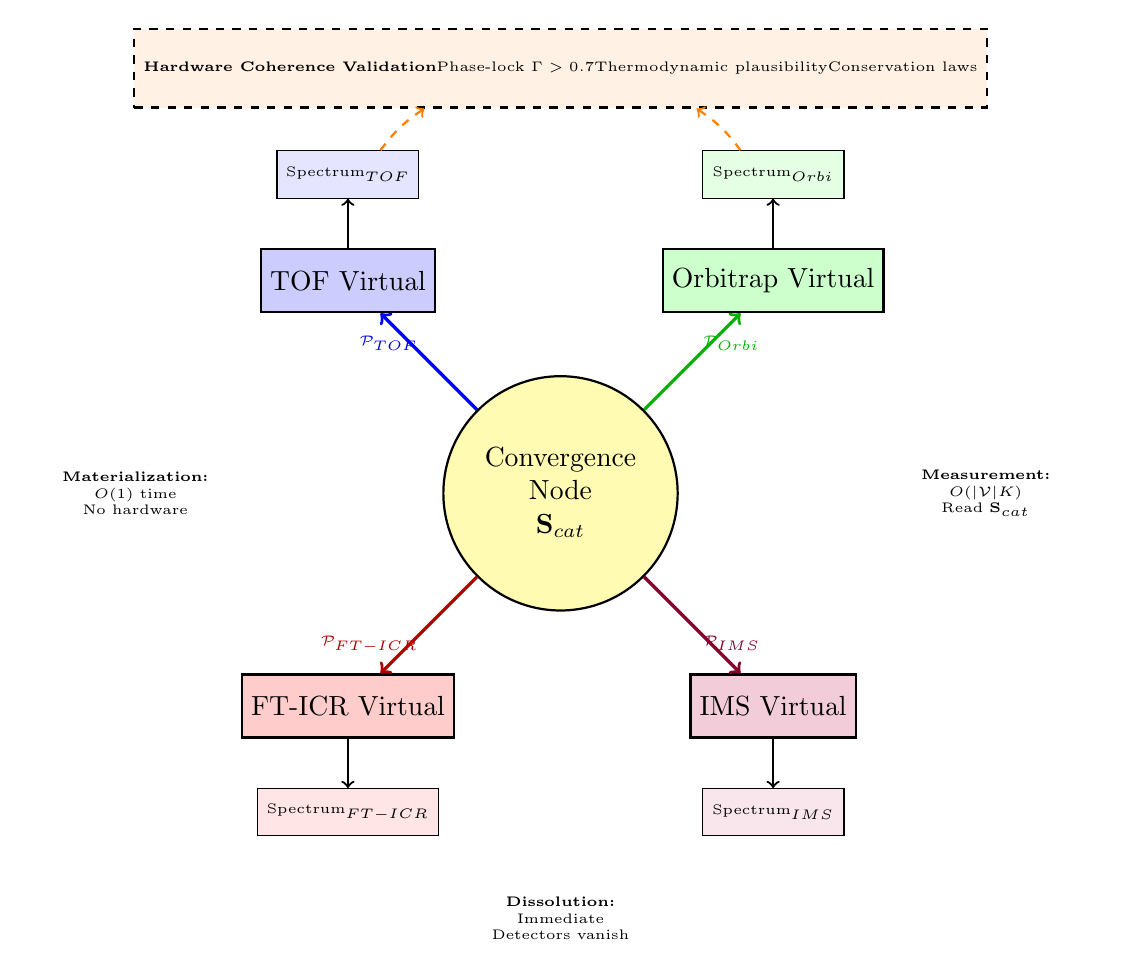
\begin{tikzpicture}[scale=0.9]
% Convergence node (center)
\node[circle, draw, thick, fill=yellow!30, minimum size=1.5cm] (CN) at (0, 0) {
\begin{tabular}{c}
Convergence\\
Node\\
$\mathbf{S}_{\text{cat}}$
\end{tabular}
};

% Virtual detectors (around node)
\node[rectangle, draw, thick, fill=blue!20, minimum width=2cm, minimum height=0.8cm] (TOF) at (-3, 3) {TOF Virtual};
\node[rectangle, draw, thick, fill=green!20, minimum width=2cm, minimum height=0.8cm] (Orbi) at (3, 3) {Orbitrap Virtual};
\node[rectangle, draw, thick, fill=red!20, minimum width=2cm, minimum height=0.8cm] (FTICR) at (-3, -3) {FT-ICR Virtual};
\node[rectangle, draw, thick, fill=purple!20, minimum width=2cm, minimum height=0.8cm] (IMS) at (3, -3) {IMS Virtual};

% Projection arrows
\draw[->, very thick, blue] (CN) -- node[above left, font=\tiny] {$\mathcal{P}_{\text{TOF}}$} (TOF);
\draw[->, very thick, green!70!black] (CN) -- node[above right, font=\tiny] {$\mathcal{P}_{\text{Orbi}}$} (Orbi);
\draw[->, very thick, red!70!black] (CN) -- node[below left, font=\tiny] {$\mathcal{P}_{\text{FT-ICR}}$} (FTICR);
\draw[->, very thick, purple!70!black] (CN) -- node[below right, font=\tiny] {$\mathcal{P}_{\text{IMS}}$} (IMS);

% Output spectra
\node[rectangle, draw, fill=blue!10, minimum width=1.8cm, minimum height=0.6cm, font=\tiny] (TOFS) at (-3, 4.5) {Spectrum$_{\text{TOF}}$};
\node[rectangle, draw, fill=green!10, minimum width=1.8cm, minimum height=0.6cm, font=\tiny] (OrbiS) at (3, 4.5) {Spectrum$_{\text{Orbi}}$};
\node[rectangle, draw, fill=red!10, minimum width=1.8cm, minimum height=0.6cm, font=\tiny] (FTICRS) at (-3, -4.5) {Spectrum$_{\text{FT-ICR}}$};
\node[rectangle, draw, fill=purple!10, minimum width=1.8cm, minimum height=0.6cm, font=\tiny] (IMSS) at (3, -4.5) {Spectrum$_{\text{IMS}}$};

\draw[->, thick] (TOF) -- (TOFS);
\draw[->, thick] (Orbi) -- (OrbiS);
\draw[->, thick] (FTICR) -- (FTICRS);
\draw[->, thick] (IMS) -- (IMSS);

% Lifecycle annotations
\node[font=\tiny, text width=2.5cm, align=center] at (-6, 0) {
\textbf{Materialization:}\\
$O(1)$ time\\
No hardware
};

\node[font=\tiny, text width=2.5cm, align=center] at (6, 0) {
\textbf{Measurement:}\\
$O(|\mathcal{V}| K)$\\
Read $\mathbf{S}_{\text{cat}}$
};

\node[font=\tiny, text width=2.5cm, align=center] at (0, -6) {
\textbf{Dissolution:}\\
Immediate\\
Detectors vanish
};

% Hardware coherence box
\node[rectangle, draw, dashed, thick, fill=orange!10, minimum width=4cm, minimum height=1cm, font=\tiny] (HC) at (0, 6) {
\textbf{Hardware Coherence Validation}\\
Phase-lock $\Gamma > 0.7$\\
Thermodynamic plausibility\\
Conservation laws
};

\draw[->, thick, dashed, orange] (TOFS) to[bend left=10] (HC);
\draw[->, thick, dashed, orange] (OrbiS) to[bend right=10] (HC);

\end{tikzpicture}
\caption{Virtual detector ensemble architecture. A single convergence node with categorical state $\mathbf{S}_{\text{cat}}$ (yellow circle) hosts four virtual detectors simultaneously. Each detector materializes, applies its projection operator ($\mathcal{P}_{\text{inst}}$), produces instrument-specific spectrum, and dissolves—all without hardware. Hardware coherence validation (orange box) ensures physical validity. All measurements are perfectly coherent (same $\mathbf{S}_{\text{cat}}$, same instant).}
\label{fig:virtual_detector_ensemble}
\end{figure}

\subsection{Comparison: Virtual vs. Physical Detectors}

\begin{table}[h]
\centering
\small
\begin{tabular}{|l|p{5cm}|p{5cm}|}
\hline
\textbf{Property} & \textbf{Physical Detector} & \textbf{Virtual Detector} \\
\hline
\textbf{Existence} & Persistent hardware (always exists) & Transient construct (exists only during measurement) \\
\hline
\textbf{Materialization time} & N/A (pre-existing) & $O(1)$ (instant) \\
\hline
\textbf{Measurement mechanism} & Physical interaction (ion hits surface, photon absorbed) & Categorical state reading (information extraction) \\
\hline
\textbf{Backaction} & Nonzero ($\Delta E > 0$, ion destroyed/perturbed) & Exactly zero ($\Delta E = 0$, state unchanged) \\
\hline
\textbf{Multi-instrument} & Sequential only (ion consumed by first detector) & Simultaneous (all instruments measure same state) \\
\hline
\textbf{Temporal coherence} & Impossible (sample changes between runs) & Perfect (same categorical state) \\
\hline
\textbf{Cost} & \$100k-\$1M+ per instrument & \$0 (computational only) \\
\hline
\textbf{Reconfigurability} & Fixed (TOF cannot become Orbitrap) & Arbitrary (change projection operator) \\
\hline
\textbf{Validation} & Calibration, maintenance, drift & Hardware coherence constraints \\
\hline
\textbf{Limitation} & Hardware specs (resolution, range, sensitivity) & Categorical state quality (convergence node density) \\
\hline
\end{tabular}
\caption{Comparison of physical and virtual detectors. Virtual detectors trade persistent hardware for transient information processing, enabling capabilities impossible with physical devices (simultaneous multi-instrument measurement, zero backaction, perfect temporal coherence).}
\label{tab:physical_vs_virtual}
\end{table}

\subsection{Summary: Virtual Detectors as Categorical State Readers}

Virtual detectors represent a paradigm shift from hardware-based measurement to information-based measurement. Key principles:

\begin{enumerate}
    \item \textbf{Transient existence}: Virtual detectors exist only during measurement, not as persistent structures (Axiom \ref{axiom:transient_existence})

    \item \textbf{Categorical state reading}: Measure by reading pre-existing categorical positions, not by physical interaction (Definition \ref{def:virtual_detector})

    \item \textbf{O(1) materialization}: Detector creation is constant-time, independent of complexity (Theorem \ref{thm:detector_lifecycle})

    \item \textbf{Instrument projections}: Different detector types are different projections of same categorical state (Theorem \ref{thm:projection_invertible})

    \item \textbf{Simultaneous multi-instrument}: Same state measured by multiple instruments simultaneously with perfect coherence (Theorem \ref{thm:simultaneous_multi_instrument})

    \item \textbf{Zero backaction}: Measurement doesn't perturb molecular system (Theorem \ref{thm:zero_backaction})

    \item \textbf{Hardware coherence}: Validation ensures physical realizability without physical hardware (Theorem \ref{thm:hardware_coherence_validity})
\end{enumerate}

This architecture enables the virtual mass spectrometry framework: multiple instruments projecting the same underlying MMD categorical state, materialized at convergence nodes, validated through hardware coherence, achieving capabilities impossible with physical detectors—all grounded in rigorous mathematical principles established in Sections 2-5.
